\documentclass{article}
\usepackage{geometry}
\geometry{
	a4paper,
	%total={170mm,257mm},
	left=20mm,
	top=30mm,
}

\usepackage{fancyhdr}
\usepackage{tikz}
\usepackage{hyperref}
\usepackage{graphicx}
\usepackage{hyperref}
\usepackage{mdframed}
\usepackage{listings} % Include the listings package
\usepackage{xcolor}   % to define your own colors
\usepackage{subcaption}

\bibliographystyle{unsrt}
\bibliography{references}


\newmdenv[
linecolor=blue, % Color of the border line
backgroundcolor=gray!20, % Background color; "gray!20" means "20% gray"
frametitle=Note, % Title of the frame, delete this line if you don't want a title
skipabove=\baselineskip, % Space above the frame
skipbelow=\baselineskip, % Space below the frame
]{mynote}

% code-snippets:
% Define the color styles you wish to use in the document for the Python syntax highlighting
\lstdefinestyle{mystyle}{
	backgroundcolor=\color{white},   % choose the background color; you must add \usepackage{color} or \usepackage{xcolor}
	commentstyle=\color{green},
	keywordstyle=\color{blue},
	numberstyle=\tiny\color{gray},
	stringstyle=\color{red},
	basicstyle=\ttfamily\footnotesize,
	breakatwhitespace=false,         
	breaklines=true,                 
	captionpos=b,                    
	keepspaces=true,                 
	numbers=left,                    
	numbersep=5pt,                  
	showspaces=false,                
	showstringspaces=false,
	showtabs=false,                  
	tabsize=2
}

\lstset{style=mystyle} % Apply your style globally to the document


\newcommand{\LVA}{Reverse Engineering}
\newcommand{\LVAKURZ}{REV3}
\newcommand{\SEMESTER}{WS 2023/2024}
\newcommand{\UELABEL}{UE 02}
\newcommand{\UETITLE}{Statische Analyse}
\newcommand{\AUTHOR}{Jakob Mayr}


\title{\vspace{5cm} \LVA\ (\LVAKURZ)\\ \vspace{1cm} \textbf{\UELABEL\ -- \UETITLE\ -- Protokoll} \vspace{2.5cm}}
\author{\AUTHOR}
\date{\SEMESTER}

\begin{document}
	
	\pagestyle{fancy}
	
	\maketitle
	
	\tikz [remember picture, overlay] %
	\node [shift={(3.7cm,-4cm)}] at (current page.north west) %
	[anchor=north west] %
	{
\includegraphics{fhooe_logo.jpg}};
	
	\tikz [remember picture, overlay] %
	\node [shift={(10cm,-4.8cm)}] at (current page.north west) %
	[anchor=north west] %
	{
\includegraphics{si_logo.jpg}};
	
	%\tikz [remember picture, overlay] %
	%\node [shift={(7.2cm,-11.65cm)}] at (current page.north west) %
	%[anchor=north west] %
	%{\includegraphics[scale=0.12]{./img/star_wars_logo_no_background.png}};
	%
	%\pagebreak
	
	\fancyhf{}
	\fancyhead[L]{\LVA\ (\LVAKURZ)}
	\fancyhead[C]{\UELABEL}
	\fancyhead[R]{\SEMESTER}
	\fancyfoot[L]{Seite \thepage\ von \pageref{LastPage}}
	\fancyfoot[R]{\AUTHOR}
	
	\section*{Einleitung}
	...\\
	
	\pagebreak
	
	\section*{Aufgabe 1 - Statische Analyse Windows}
	\subsection*{Erstellen der Dateien}
	In Aufgabe 1 ist eine Anwendung, welche "infected" auf \texttt{stdout} ausgibt in \texttt{c} zu schreiben und mit Visual Studio auf 4 verschiedene Varianten zu bauen.\\
	Die vier Varianten mit deren Eigenschaften und Unterschieden (Quelle: \href{https://chat.openai.com}{ChatGPT}):\\
	\begin{enumerate}
		\item \textbf{Static Release (/MT)}:
		\begin{enumerate}
			\item Laufzeitbibliothek: Statisch
			\item Debug-Informationen: Nein
			\item Eigenschaften:
			\begin{enumerate}
				\item Die Laufzeitbibliothek wird in die ausführbare Datei eingebettet.
				\item Größere Dateigröße, da der Code der CRT (C Runtime Library) direkt in die Anwendung eingefügt wird.
				\item Keine Abhängigkeit von DLLs (Dynamically Linked Libraries) zur Laufzeit.
				\item Optimiert für Geschwindigkeit und nicht für das Debugging.
			\end{enumerate}
		\end{enumerate}
		\item \textbf{Static Debug (/MTd)}:
		\begin{enumerate}
			\item Laufzeitbibliothek: Statisch
			\item Debug-Informationen: Ja
			\item Eigenschaften:
			\begin{enumerate}
				\item Ähnlich wie /MT, aber mit zusätzlichen Debug-Informationen und weniger Optimierungen.
				\item Erleichtert das Debugging, da Variablen leichter überwacht werden können.
				\item Größerer Speicherbedarf und langsamere Ausführung im Vergleich zur Release-Version.
			\end{enumerate}
		\end{enumerate}
		\item \textbf{Dynamic Relase (/MD)}:
		\begin{enumerate}
			\item Laufzeitbibliothek: Dynamisch
			\item Debug-Informationen: Nein
			\item Eigenschaften:
			\begin{enumerate}
				\item Verlinkt dynamisch mit den CRT-DLLs (Z.B. msvcrXXX.dll).
				\item Kleinere Dateigröße, da die Laufzeitbibliothek nicht eingebettet ist.
				\item Erfordert, dass die CRT-DLLs zur Laufzeit verfügbar sind.
				\item Optimiert für Geschwindigkeit.
			\end{enumerate}
		\end{enumerate}
		\item \textbf{Dynamic Debug (/MDd)}:
		\begin{enumerate}
			\item Laufzeitbibliothek: Dynamisch
			\item Debug-Informationen: Ja
			\item Eigenschaften:
			\begin{enumerate}
				\item Ähnlich wie /MD, aber mit zusätzlichen Debug-Informationen und weniger Optimierungen.
				\item Erleichter das Debugging.
				\item Erfodert, dass die Debug-Version der CRT-DLLs zur Laufzeit verfügbar ist.
			\end{enumerate}
		\end{enumerate}
	\end{enumerate}
	
	\pagebreak
	
	\textbf{Unterschiede:}\\
	\begin{enumerate}
		\item \textbf{Statische vs. Dynamische Verlinkung}: /MT und /MTd binden die Laufzeitbibliothek statisch ein, wodurch die ausführbare Datei unabhängig von externen DLLs ist. /MD und /MDd verlinken dynamisch und erfordern, dass die entsprechenden DLLs zur Laufzeit vorhanden sind.
		\item \textbf{Debug vs. Release}: Die Debug-Optionen (/MTd und /MDd) enthalten zusätzliche Debug-Informationen und sind nicht so stark optimiert wie die Release-Optionen (/MT und /MD), was das Debugging erleichtert, aber die Leistung beeinträchtigen kann. 
	\end{enumerate}
	
	\noindent \textbf{Der Programm-Code für die gewünschte Executable:}\\
	\begin{lstlisting}[language=c]
		#include <stdio.h>
		
		int main() {
			printf("infected");
			return = 0;
		}
	\end{lstlisting}
	In den Einstellungen des Visual Studio Projekts kann die gewünschte Variante für die "Runtime Library" ausgewählt werden:\\
	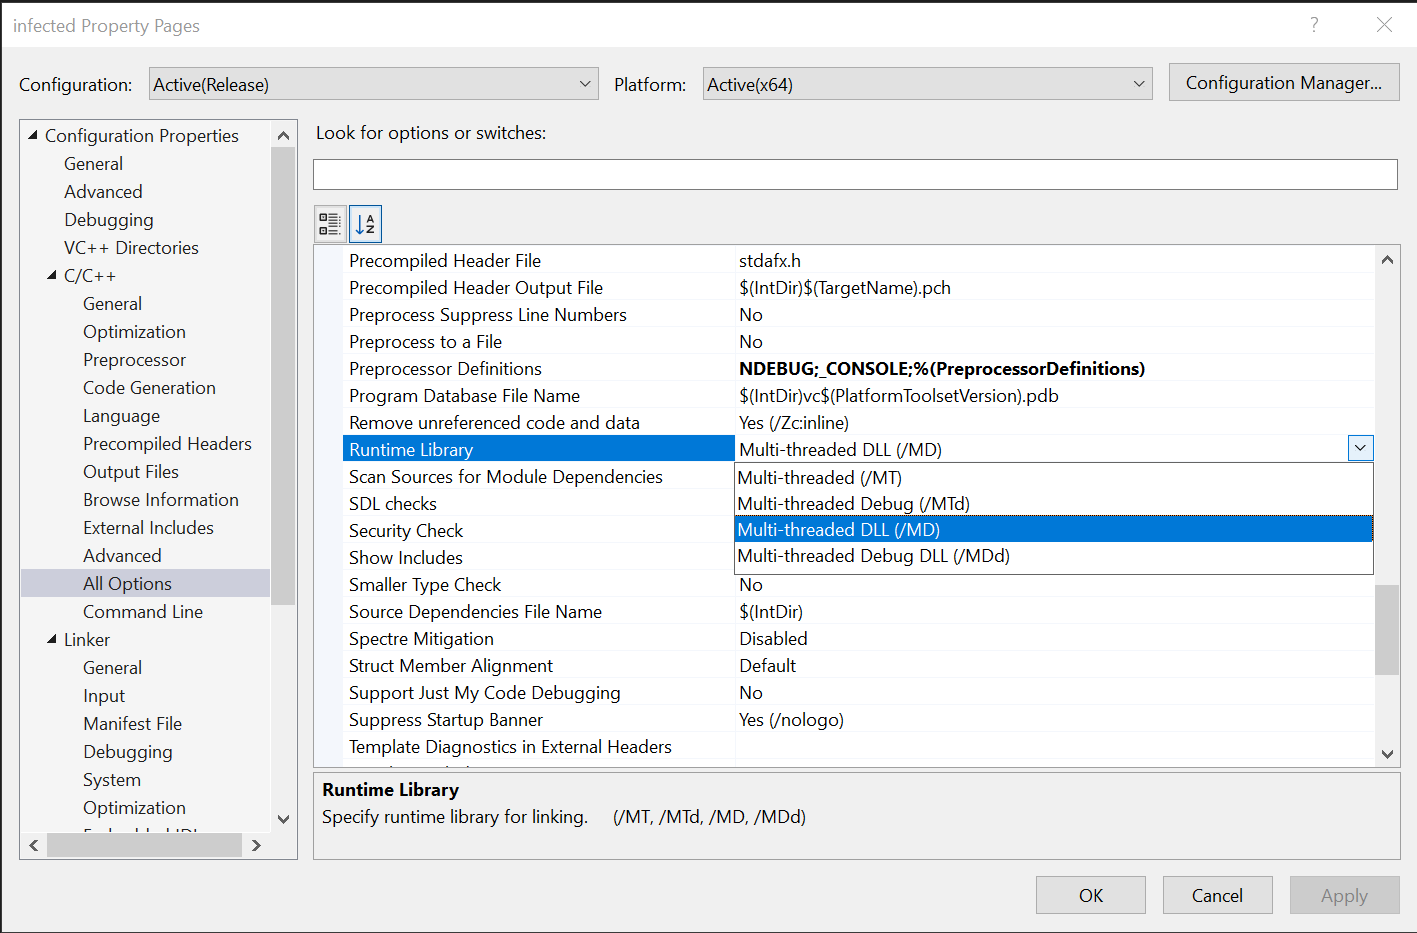
\includegraphics[width=0.7\linewidth]{pictures/1. setting runtime library.png}\\
	Die Files nach erstellen, hier ist direkt ersichtlich, dass beide statischen Varianten größer sind (Length), da sich der Code der Libraries im File befindet:\\
	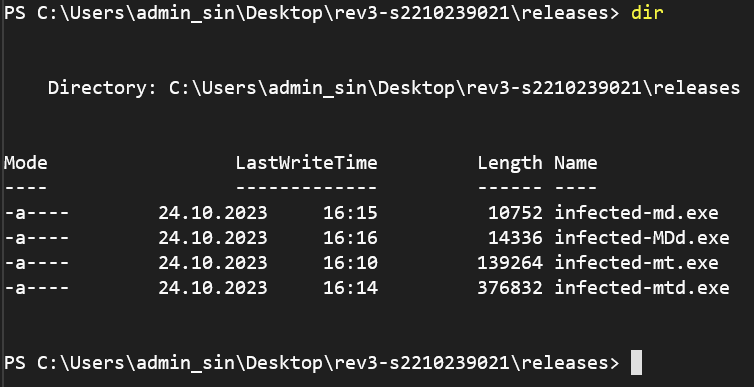
\includegraphics[width=0.5\linewidth]{pictures/1. all files.png}\\
	
	\pagebreak
	\subsection*{Analyse der Dateien}
	Um die erzeugten Executables zu analysieren sollen zumindest die Tools \texttt{dumpbin} und \texttt{strings} verwendet werden.\\
	\subsection*{dumpbin}
	\texttt{dumpbin} ist ein Command-Line Tool, zur Verfügung gestellt von \texttt{Microsoft Visual Studio} um PE-Files (Portable Executable) zu analysieren. Es können beispielsweise die flags \textbf{/DEPENDENTS}, \textbf{/EXPORTS}, \textbf{/HEADERS} oder \textbf{/ALL} verwendet werden, um alle vom Tool lieferbaren Informationen zu erhalten.\\
	
	\noindent Folgende Aufrufe zeigen die Ausgabe ohne Parameter:\\
	\begin{figure}[htp]
		\centering
		\begin{subfigure}[b]{0.45\textwidth}
			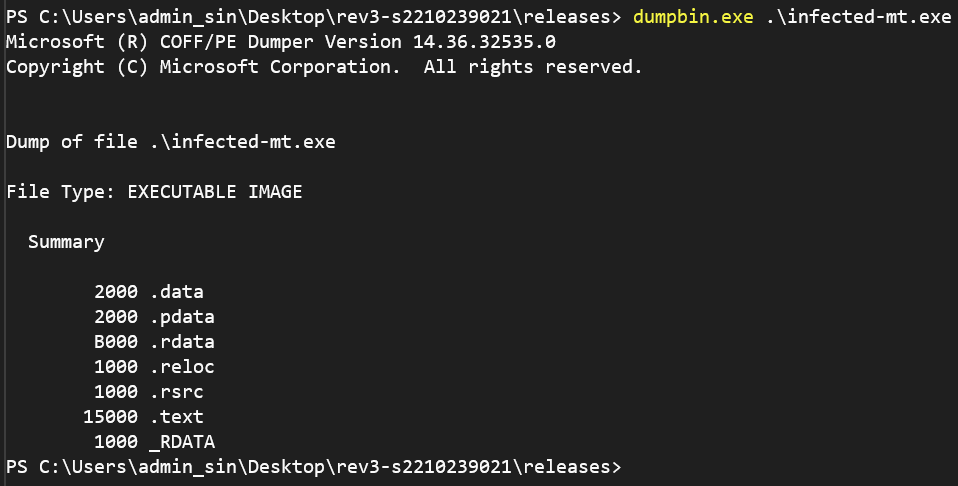
\includegraphics[width=\textwidth]{pictures/1. dumpbin mt.png}
			\caption{dumpbin mt-file}
			\label{fig:image1}
		\end{subfigure}
		\hfill
		\begin{subfigure}[b]{0.45\textwidth}
			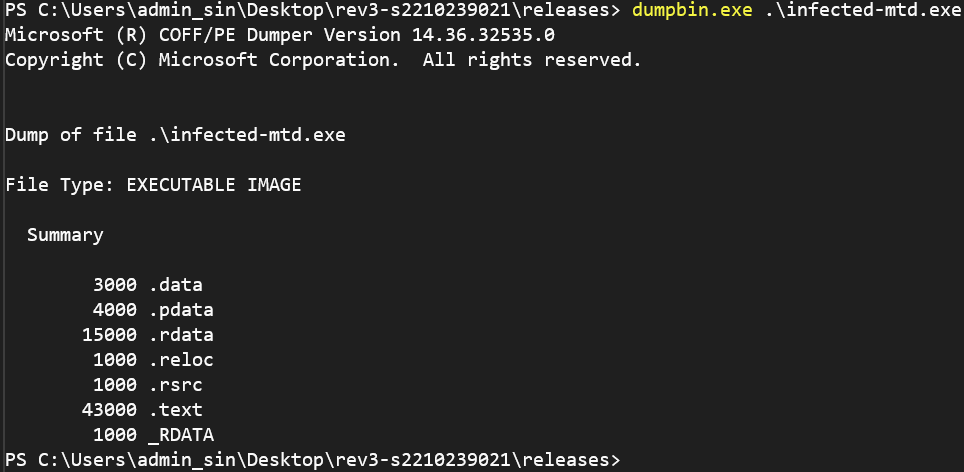
\includegraphics[width=\textwidth]{pictures/1. dumpbin mtd.png}
			\caption{dumpbin mtd-file}
			\label{fig:image2}
		\end{subfigure}
		
		\vspace{10pt} % Adjust to your liking
		
		\begin{subfigure}[b]{0.45\textwidth}
			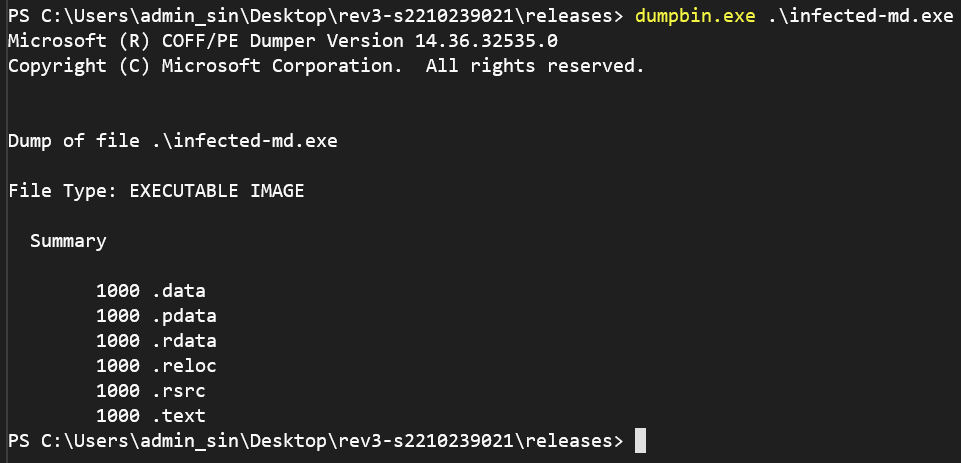
\includegraphics[width=\textwidth]{pictures/1. dumpbin md.png}
			\caption{dumpbin md-file}
			\label{fig:image3}
		\end{subfigure}
		\hfill
		\begin{subfigure}[b]{0.45\textwidth}
			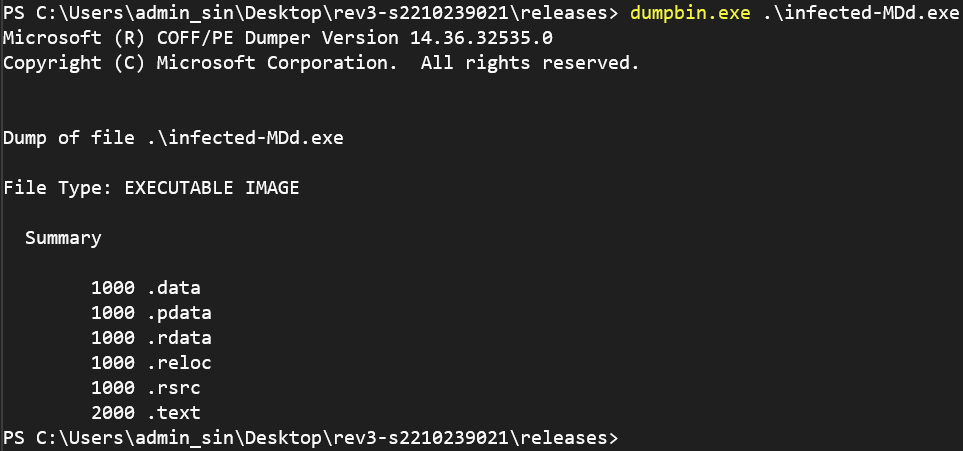
\includegraphics[width=\textwidth]{pictures/1. dumpbin mdd.png}
			\caption{dumpbin mdd-file}
			\label{fig:image4}
		\end{subfigure}
		\caption{All infected.exe files analysed with dumpbin}
		\label{fig:grid}
	\end{figure}
	
	\noindent Die Debug-Versionen (infected-MDd.exe und infected-mtd.exe) haben tendenziell größere .text Sektionen als ihre entsprechenden Release-Versionen, da sie zusätzliche Debug-Informationen enthalten.\\
	Die statisch verlinkten Versionen (infected-mt.exe und infected-mtd.exe) haben größere .text und .rdata Sektionen im Vergleich zu den dynamisch verlinkten Versionen, da die C Runtime Library direkt in die ausführbare Datei eingebettet ist.\\
	Die dynamisch verlinkten Versionen (infected-md.exe und infected-MDd.exe) sind im Allgemeinen kleiner, weil sie zur Laufzeit externe DLLs verwenden.\\
	
	\pagebreak
	
	\subsection*{strings}
	Der Befehl strings wird verwendet, um alle druckbaren Zeichenfolgen in einer Binärdatei zu extrahieren und anzuzeigen. Eine Zeichenfolge in diesem Kontext ist eine Sequenz von druckbaren Zeichen, die typischerweise durch Null-Bytes (\textbackslash0) oder durch nicht-druckbare Zeichen getrennt ist. Dieses Tool ist nützlich, um Text, Pfade, URLs, Versionen und andere Informationen aus ausführbaren Dateien, Bibliotheken oder beliebigen Binärdateien zu extrahieren.\\
	Folgende zwei screenshots zeigen sowohl den Anfang als auch das Ende der 4 verscheidenen Files:\\
	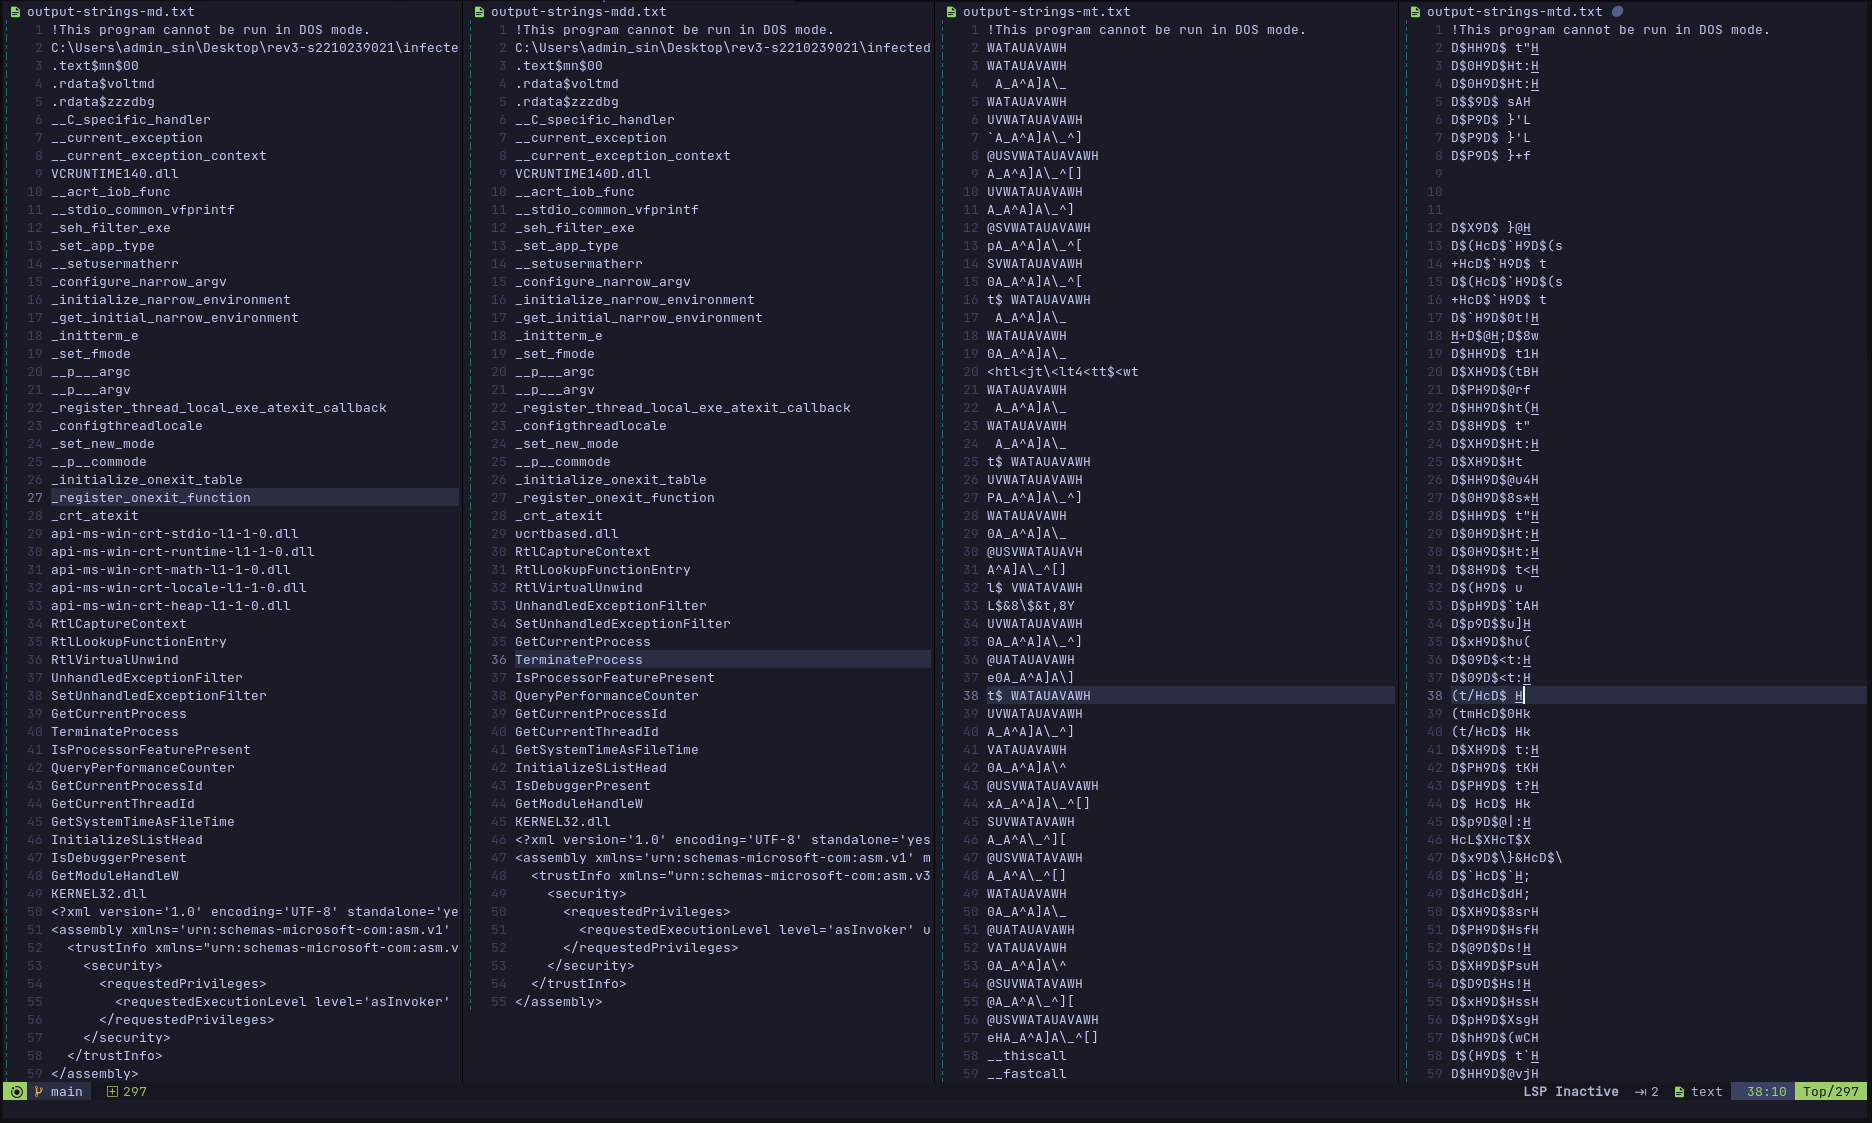
\includegraphics[width=1\linewidth]{pictures/1. strings from all files}\\
	\\
	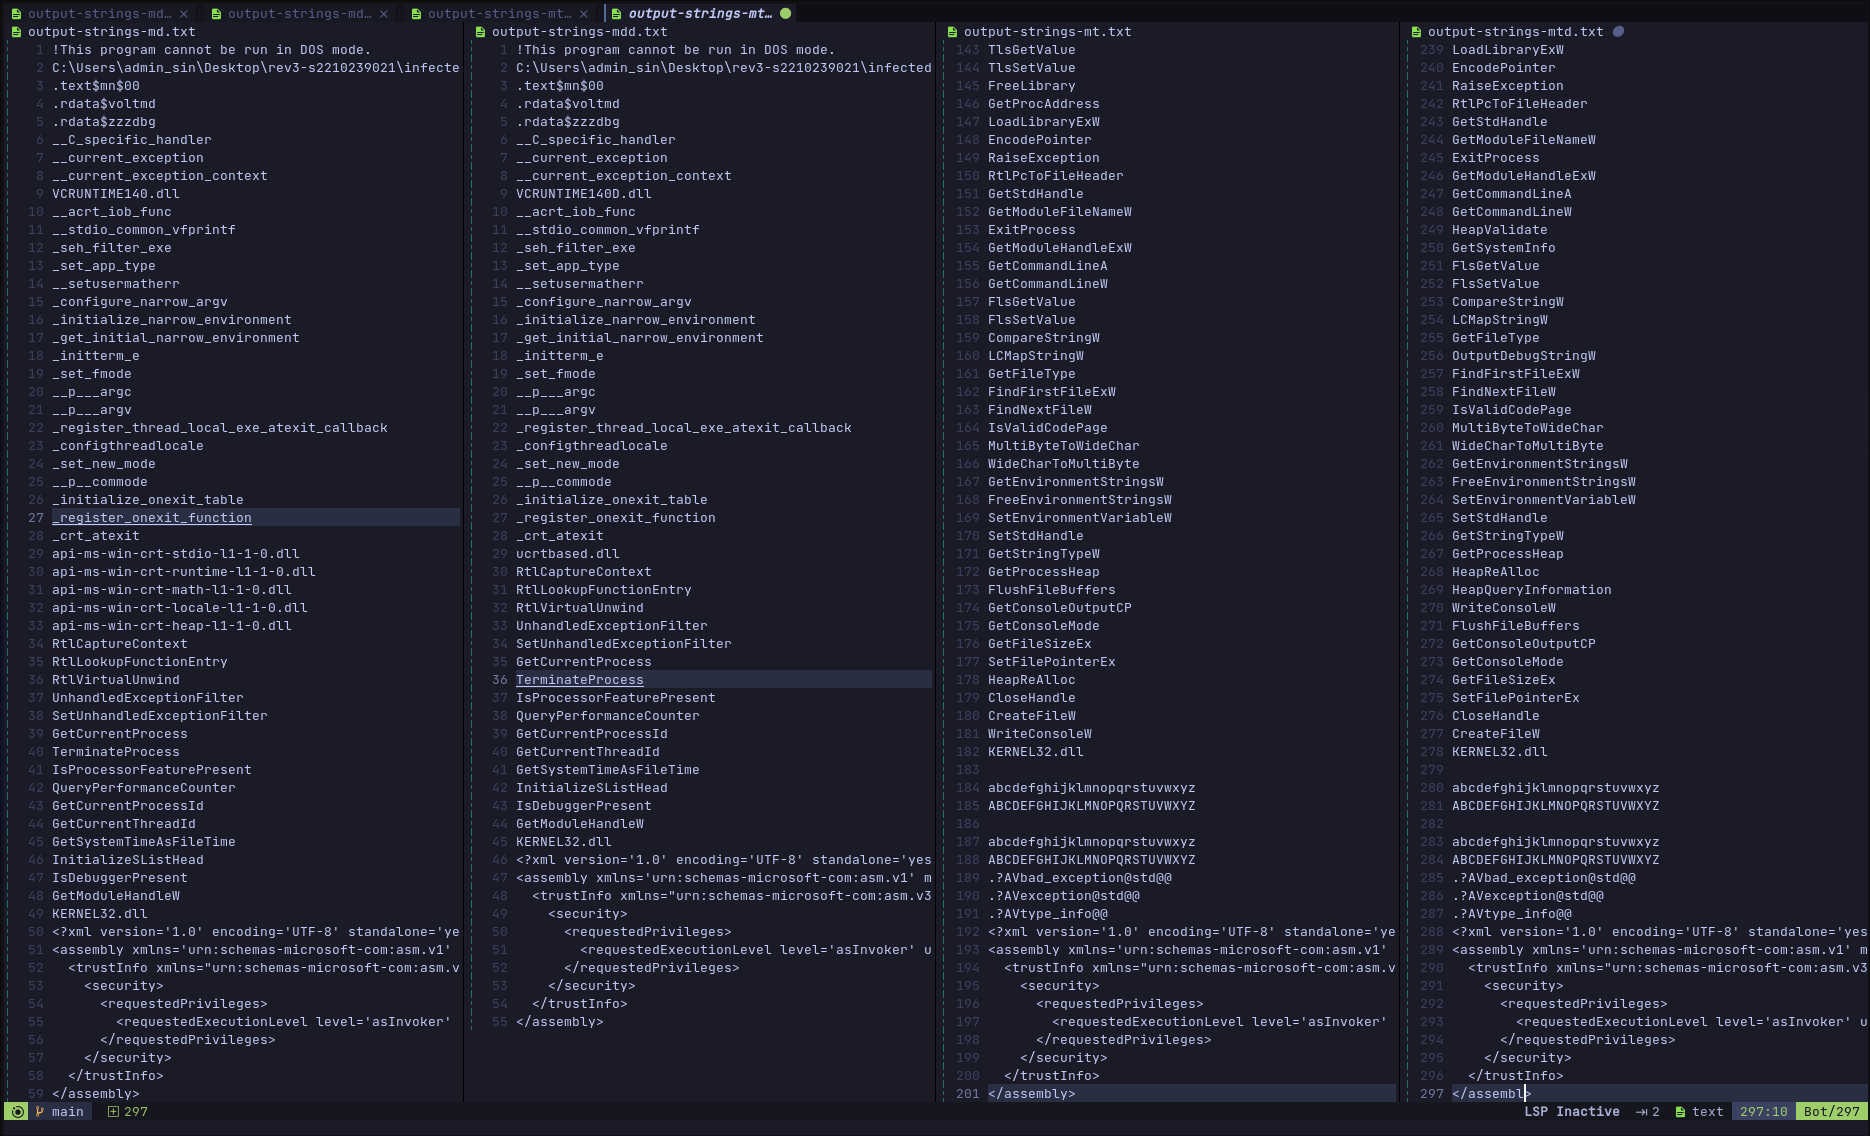
\includegraphics[width=1\linewidth]{pictures/1. strings from all files.2}\\
	
	\subsection*{Fragen}
	\begin{enumerate}
		\item \textbf{Welche Imports werden verwendet?}\\
		Durch den Aufruf von \texttt{dumpbin /IMPORTS <PE-filename>} können die Imports ermittelt werden:\\
		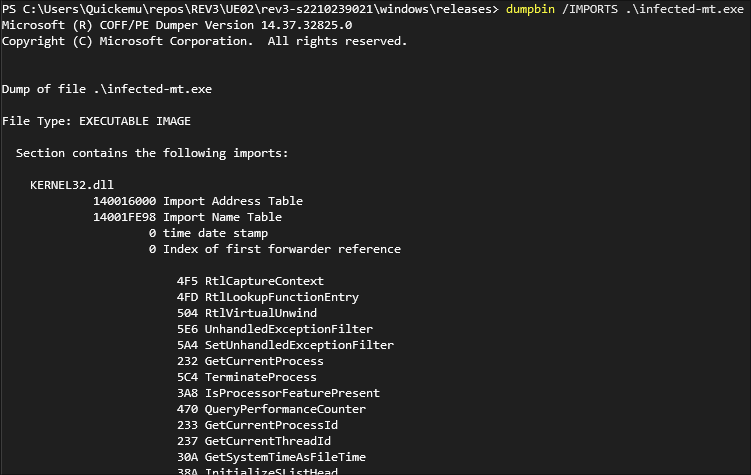
\includegraphics[width=1\linewidth]{pictures/1. example imports}
		\begin{enumerate}
			\item infected-mt.exe
			\begin{enumerate}
				\item KERNEL32.dll
			\end{enumerate}
			\item infected-mtd.exe
			\begin{enumerate}
				\item KERNEL32.dll
			\end{enumerate}
			\item infected-md.exe
			\begin{enumerate}
				\item VCRUNTIME140.dll
				\item api-ms-win-crt-stdio-l1-1-0.dll
				\item api-ms-win-crt-runtime-l1-1-0.dll
				\item api-ms-win-crt-math-l1-1-0.dll
				\item api-ms-win-crt-locale-l1-1-0.dll
				\item api-ms-win-crt-heap-l1-1-0.dll
				\item KERNEL32.dll
			\end{enumerate}
			\item infected-MDd.exe
			\begin{enumerate}
				\item VCRUNTIME140D.dll
				\item ucrtbased.dll
				\item KERNEL32.dll
			\end{enumerate}
		\end{enumerate}
		\pagebreak
		\item \textbf{Welche Sektionen werden verwedent?}\\
		Durch den Aufruf von \texttt{dumpbin <PE-filename>} können die Sektionen ermittelt werden:\\
		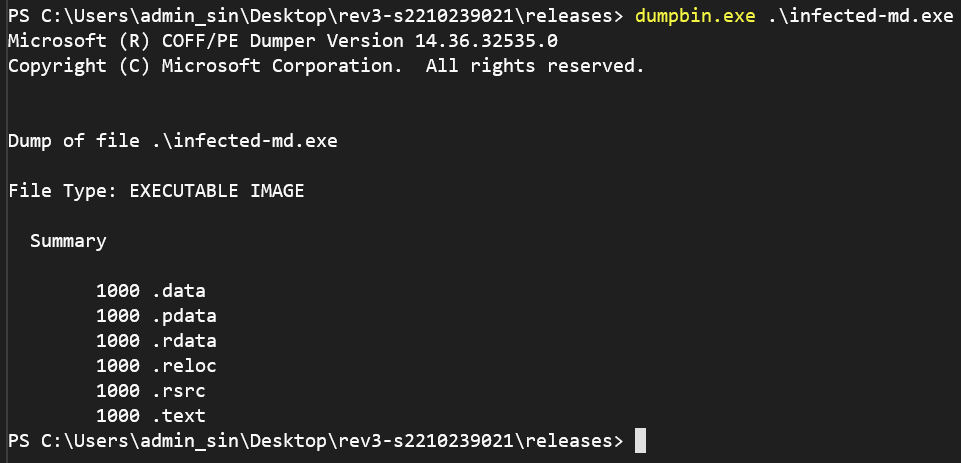
\includegraphics[width=1\linewidth]{pictures/1. dumpbin md}
		\begin{enumerate}
			\item infected-mt.exe
			\begin{enumerate}
				\item .text
				\item .rdata
				\item .data
				\item .pdata
				\item \_RDATA
				\item .rsrc
				\item .reloc
			\end{enumerate}
			\item infected-mtd.exe
			\begin{enumerate}
				\item .text
				\item .rdata
				\item .data
				\item .pdata
				\item \_RDATA
				\item .rsrc
				\item .reloc
			\end{enumerate}
			\item infected-md.exe
			\begin{enumerate}
				\item .text
				\item .rdata
				\item .data
				\item .pdata
				\item .rsrc
				\item .reloc
			\end{enumerate}
			\item infected-MDd.exe
			\begin{enumerate}
				\item .text
				\item .rdata
				\item .data
				\item .pdata
				\item .rsrc
				\item .reloc
			\end{enumerate}
		\end{enumerate}
		
		\pagebreak
		
		\item \textbf{Was kannst du über die*den Author*in sagen?}
		Ein direkter Author ist nicht erkennbar. Allerdings könnte man auf "admin\_sin" schließen, da das File für die "Program Database" (infected.pbd) im Pfad den User nennt:\\
		\begin{lstlisting}[language=c]
			 Debug Directories
			
			Time Type        Size      RVA  Pointer
			-------- ------- -------- -------- --------
			6537D1B0 cv            66 00003464     2264    Format: RSDS, {6F72B84A-D687-4743-A104-E88EF40E7E96}, 4, C:\Users\admin_sin\Desktop\rev3-s2210239021\infected\x64\Release\infected.pdb
			6537D1B0 feat          14 000034CC     22CC    Counts: Pre-VC++ 11.00=0, C/C++=30, /GS=30, /sdl=1, guardN=29
			6537D1B0 coffgrp      284 000034E0     22E0    4C544347 (LTCG)
			6537D1B0 iltcg          0 00000000        0
			
		\end{lstlisting}
		
		\noindent Dies ist in allen Files gleich herauszulesen.\\
		
		\item \textbf{Was kannst du über die Umgebung, in der das Sample erzeugt wurde, sagen?}\\
		Auskünfte über die Umgebung können durch die Compiler-Version, eingebettete Ressourcen oder Abhängigkeiten und der Weiteren gegeben werden.\\
		\textbf{HEADERS}\\
		Durch den Aufruf von \texttt{dumpbin /HEADERS <PE-filename>} können mehrere Informationen über die Umgebung herausgefunden werden:\\
		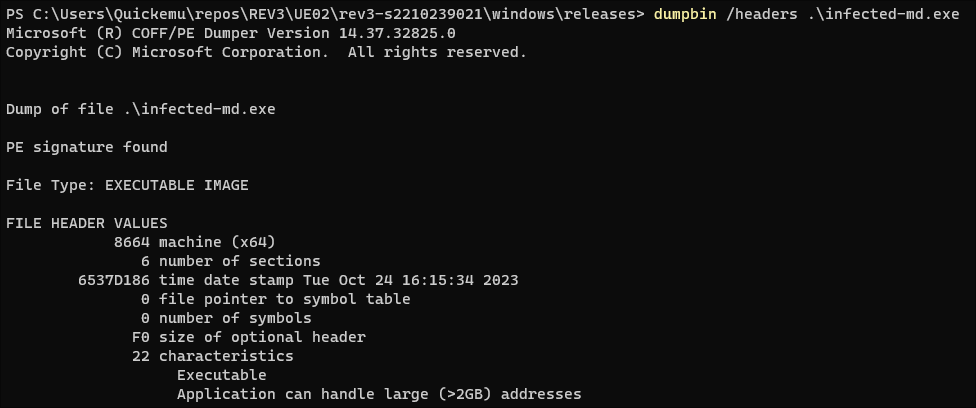
\includegraphics[width=1\linewidth]{pictures/1. umgebung}\\
		(Der Screenshot zeigt nur den Beginn des outputs...)\\
		Folgende Informationen können über die Files gefunden werden:\\
		\begin{enumerate}
			\item infected-mt.exe
			\begin{enumerate}
				\item \textbf{Architektur:} 8664 machine (x64)
				\item \textbf{Linker-Version}: 14.36 (typisch für Visual Studio-Version)
				\item \textbf{Zeitstempel}: Tue Oct 24 16:10:20 2023
				\item \textbf{Subsystem}: Windows CUI (Konsolenanwendung)
				\item \textbf{DLL-Charakteristika}:\\
				Kompatibel mit "High Entropy Virtual Addresses", "Dynamic Base", "NX (No eXecute)", "Terminal Server Aware".\\
				Diese Eigenschaften sind Sicherheitsmerkmale, die oft in modernen Anwendungen verwendet werden.
				\item Speicherreservierung: Die Größen für Stack- und Heap-Reservierung und -Commit sind angegeben, was Hinweise auf den für die Ausführung der Anwendung benötigten Speicher gibt.
				\item \textbf{Verzeichnisse und Sektionen}: Verschiedene Verzeichnisse wie das Importverzeichnis, das Resourceverzeichnis, das Exceptionverzeichnis usw. sind aufgelistet. Diese geben Informationen über die Struktur der ausführbaren Datei und welche externen Funktionen oder Ressourcen sie verwendet.\\
				Beispielseweise nur für mt-Version angeführt:\\
				\begin{lstlisting}[language=c]
						              10 number of directories
						0 [       0] RVA [size] of Export Directory
						28DC [      A0] RVA [size] of Import Directory
						5000 [     1E0] RVA [size] of Resource Directory
						4000 [     174] RVA [size] of Exception Directory
						0 [       0] RVA [size] of Certificates Directory
						6000 [      30] RVA [size] of Base Relocation Directory
						23A0 [      70] RVA [size] of Debug Directory
						0 [       0] RVA [size] of Architecture Directory
						0 [       0] RVA [size] of Global Pointer Directory
						0 [       0] RVA [size] of Thread Storage Directory
						2260 [     140] RVA [size] of Load Configuration Directory
						0 [       0] RVA [size] of Bound Import Directory
						2000 [     1A0] RVA [size] of Import Address Table Directory
						0 [       0] RVA [size] of Delay Import Directory
						0 [       0] RVA [size] of COM Descriptor Directory
						0 [       0] RVA [size] of Reserved Directory
				\end{lstlisting}
				\item \textbf{Betriebssystem- und Subsystem-Version}: Das Betriebssystem und das Subsystem sind auf Version 6.00 eingestellt. Dies könnte auf eine Kompatibilität mit bestimmten Windows-Versionen hinweisen (z.B. Windows Vista, 7, 8, 10), die alle NT 6.x-Versionen sind.
				\item \textbf{Art der Ausführbaren}: Die Ausführbare ist als "Executable" markiert, was darauf hindeutet, dass es sich um eine Standard-Ausführbare (und nicht um eine DLL) handelt.
			\end{enumerate}
			\item infected-mtd.exe
			\begin{enumerate}
				\item \textbf{Architektur:} 8664 machine (x64)
				\item \textbf{Linker-Version}: 14.36 (typisch für Visual Studio-Version)
				\item \textbf{Zeitstempel}: Tue Oct 24 16:14:17 2023
				\item \textbf{Subsystem}: Windows CUI (Konsolenanwendung)
				\item \textbf{DLL-Charakteristika}:\\
				Kompatibel mit "High Entropy Virtual Addresses", "Dynamic Base", "NX (No eXecute)", "Terminal Server Aware".\\
				Diese Eigenschaften sind Sicherheitsmerkmale, die oft in modernen Anwendungen verwendet werden.
				\item Speicherreservierung: Die Größen für Stack- und Heap-Reservierung und -Commit sind angegeben, was Hinweise auf den für die Ausführung der Anwendung benötigten Speicher gibt.
				\item \textbf{Verzeichnisse und Sektionen}: Verschiedene Verzeichnisse wie das Importverzeichnis, das Resourceverzeichnis, das Exceptionverzeichnis usw. sind aufgelistet. Diese geben Informationen über die Struktur der ausführbaren Datei und welche externen Funktionen oder Ressourcen sie verwendet.
				\item \textbf{Betriebssystem- und Subsystem-Version}: Das Betriebssystem und das Subsystem sind auf Version 6.00 eingestellt. Dies könnte auf eine Kompatibilität mit bestimmten Windows-Versionen hinweisen (z.B. Windows Vista, 7, 8, 10), die alle NT 6.x-Versionen sind.
				\item \textbf{Art der Ausführbaren}: Die Ausführbare ist als "Executable" markiert, was darauf hindeutet, dass es sich um eine Standard-Ausführbare (und nicht um eine DLL) handelt.
			\end{enumerate}
			\item infected-md.exe
			\begin{enumerate}
				\item \textbf{Architektur:} 8664 machine (x64)
				\item \textbf{Linker-Version}: 14.36 (typisch für Visual Studio-Version)
				\item \textbf{Zeitstempel}: Tue Oct 24 16:15:34 2023
				\item \textbf{Subsystem}: Windows CUI (Konsolenanwendung)
				\item \textbf{DLL-Charakteristika}:\\
				Kompatibel mit "High Entropy Virtual Addresses", "Dynamic Base", "NX (No eXecute)", "Terminal Server Aware".\\
				Diese Eigenschaften sind Sicherheitsmerkmale, die oft in modernen Anwendungen verwendet werden.
				\item Speicherreservierung: Die Größen für Stack- und Heap-Reservierung und -Commit sind angegeben, was Hinweise auf den für die Ausführung der Anwendung benötigten Speicher gibt.
				\item \textbf{Verzeichnisse und Sektionen}: Verschiedene Verzeichnisse wie das Importverzeichnis, das Resourceverzeichnis, das Exceptionverzeichnis usw. sind aufgelistet. Diese geben Informationen über die Struktur der ausführbaren Datei und welche externen Funktionen oder Ressourcen sie verwendet.
				\item \textbf{Betriebssystem- und Subsystem-Version}: Das Betriebssystem und das Subsystem sind auf Version 6.00 eingestellt. Dies könnte auf eine Kompatibilität mit bestimmten Windows-Versionen hinweisen (z.B. Windows Vista, 7, 8, 10), die alle NT 6.x-Versionen sind.
				\item \textbf{Art der Ausführbaren}: Die Ausführbare ist als "Executable" markiert, was darauf hindeutet, dass es sich um eine Standard-Ausführbare (und nicht um eine DLL) handelt.
			\end{enumerate}
			\item infected-MDd.exe
			\begin{enumerate}
				\item \textbf{Architektur:} 8664 machine (x64)
				\item \textbf{Linker-Version}: 14.36 (typisch für Visual Studio-Version)
				\item \textbf{Zeitstempel}: Tue Oct 24 16:16:16 2023
				\item \textbf{Subsystem}: Windows CUI (Konsolenanwendung)
				\item \textbf{DLL-Charakteristika}:\\
				Kompatibel mit "High Entropy Virtual Addresses", "Dynamic Base", "NX (No eXecute)", "Terminal Server Aware".\\
				Diese Eigenschaften sind Sicherheitsmerkmale, die oft in modernen Anwendungen verwendet werden.
				\item Speicherreservierung: Die Größen für Stack- und Heap-Reservierung und -Commit sind angegeben, was Hinweise auf den für die Ausführung der Anwendung benötigten Speicher gibt.
				\item \textbf{Verzeichnisse und Sektionen}: Verschiedene Verzeichnisse wie das Importverzeichnis, das Resourceverzeichnis, das Exceptionverzeichnis usw. sind aufgelistet. Diese geben Informationen über die Struktur der ausführbaren Datei und welche externen Funktionen oder Ressourcen sie verwendet.
				\item \textbf{Betriebssystem- und Subsystem-Version}: Das Betriebssystem und das Subsystem sind auf Version 6.00 eingestellt. Dies könnte auf eine Kompatibilität mit bestimmten Windows-Versionen hinweisen (z.B. Windows Vista, 7, 8, 10), die alle NT 6.x-Versionen sind.
				\item \textbf{Art der Ausführbaren}: Die Ausführbare ist als "Executable" markiert, was darauf hindeutet, dass es sich um eine Standard-Ausführbare (und nicht um eine DLL) handelt.
			\end{enumerate}
		\end{enumerate}
		Unterschiede in den Versionen finden sich in der Anzahl der Sektionen, dem Zeitstempel, der größe des Codes, der Relativ Virtuellen Adresse (RVA) sowie der größe verschiedener Verzeichnisse (Import Directory, Resource Directory, Exception Directory, Base Relocation Directory, Debug Directory, Load Configuration Directory, Import Address Table Directory)  wieder. Ebenfalls unterscheidet sich die Anzahl der Verzeichnisse.\\
	\end{enumerate}
	
	\pagebreak
	
	\noindent \textbf{DEPENDENCIES}\\
	Durch den Aufruf von \texttt{dumpbin /DEPENDECIES <PE-filename>} können mehrere Informationen über die Umgebung herausgefunden werden:\\
	\begin{figure}[htp]
		\centering
		\begin{subfigure}[b]{0.45\textwidth}
			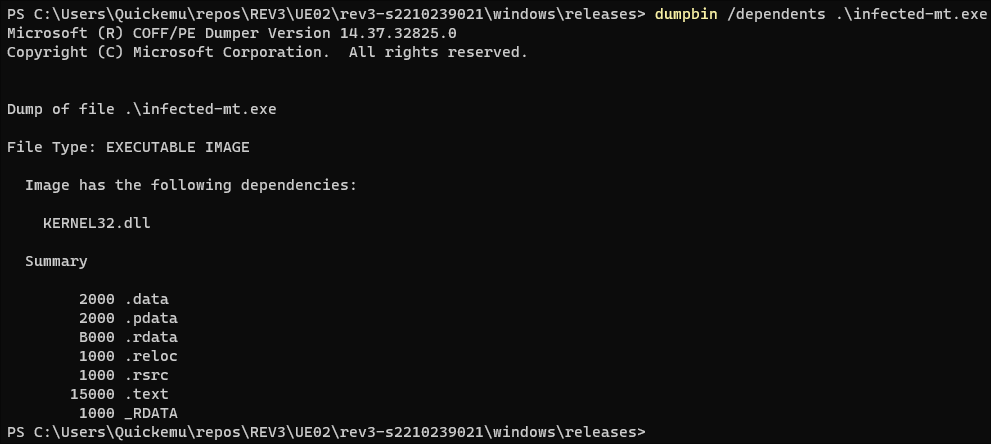
\includegraphics[width=\textwidth]{pictures/1. dependencies-mt.png}
			\caption{dependencies mt-file}
			\label{fig:image1}
		\end{subfigure}
		\hfill
		\begin{subfigure}[b]{0.45\textwidth}
			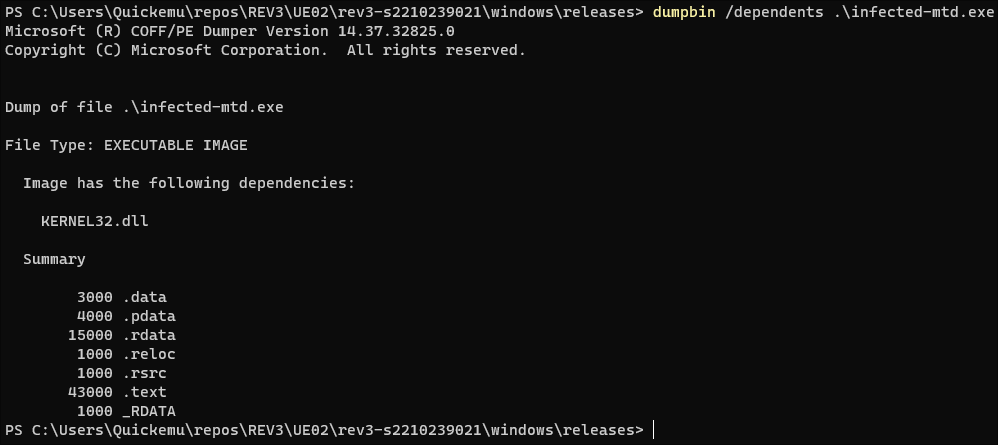
\includegraphics[width=\textwidth]{pictures/1. dependencies-mtd.png}
			\caption{dependencies mtd-file}
			\label{fig:image2}
		\end{subfigure}
		
		\vspace{10pt} % Adjust to your liking
		
		\begin{subfigure}[b]{0.45\textwidth}
			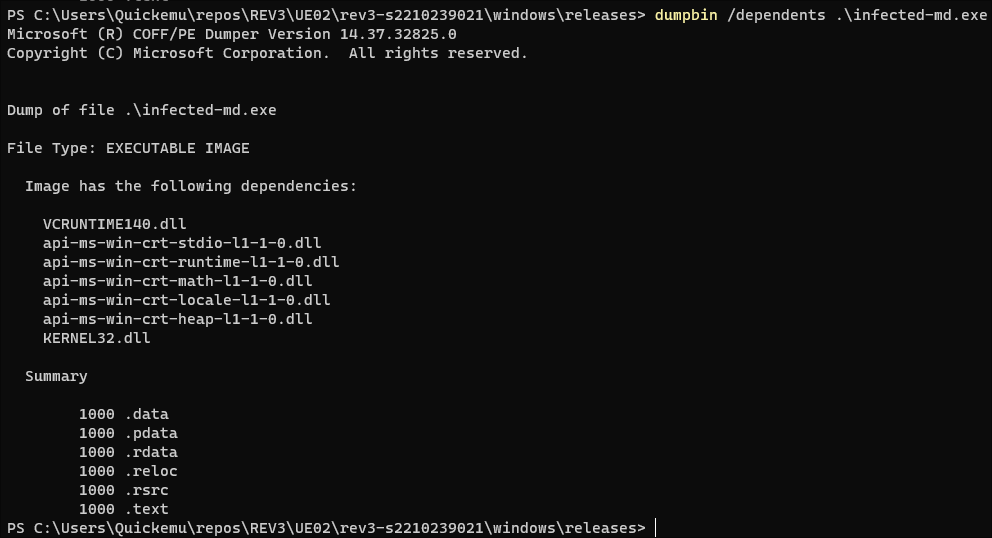
\includegraphics[width=\textwidth]{pictures/1. dependencies-md.png}
			\caption{dependencies md-file}
			\label{fig:image3}
		\end{subfigure}
		\hfill
		\begin{subfigure}[b]{0.45\textwidth}
			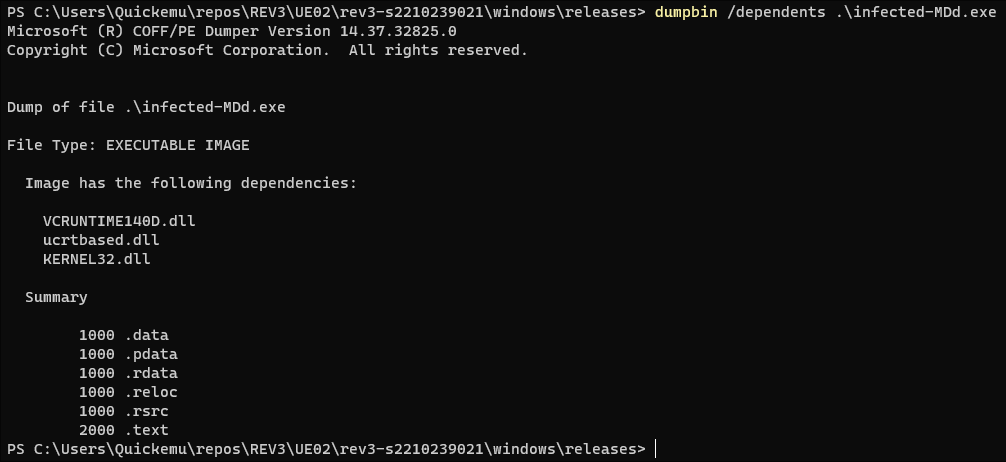
\includegraphics[width=\textwidth]{pictures/1. dependencies-mdd.png}
			\caption{dependencies mdd-file}
			\label{fig:image4}
		\end{subfigure}
		\caption{All dependencies}
		\label{fig:grid}
	\end{figure}
	
	Die Unterschiedlichen Abhängigkeiten geben ebenfalls Auskunft über die Umgebung.\\
	
	\noindent \textbf{Weitere Informationen zur Umgebung}\\
	Es können natürlich noch weitere Informationen über die Umgebung gefunden werden, hilfreich können auch die Parameter \texttt{/DEBUG}, \texttt{/IMPORTS} oder \texttt{/RESSOURCES} sein, es kommt jedoch immer darauf an, wonach gesucht wird.\\
	
	
	\pagebreak
	
	\section*{2. Aufgabe - Statische Analyse Linux}
	\subsection*{create file}
	Gleicher code wie zuvor:\\
	\begin{lstlisting}[language=c]
		#include <stdio.h>
		
		int main() {
			printf("infected");
			return = 0;
		}
	\end{lstlisting}
	Kompilieren und auflisten der Executables:\\
	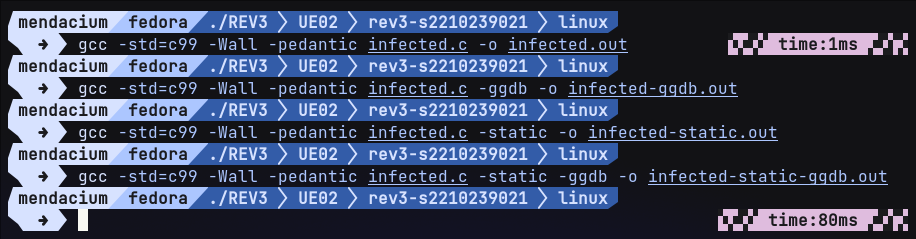
\includegraphics[width=0.7\linewidth]{pictures/2. compile files}\\
	\\
	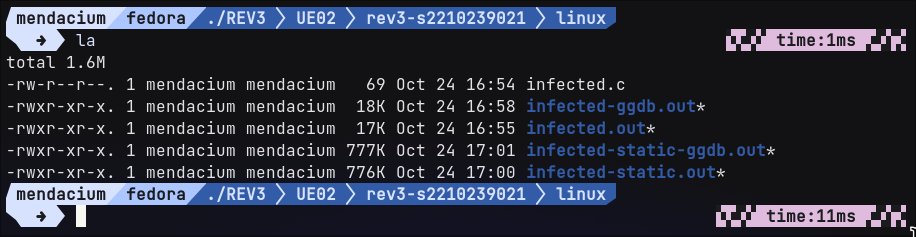
\includegraphics[width=0.5\linewidth]{pictures/2. all files}\\
	
	\subsection*{Fragen}
	\begin{enumerate}
		\item \textbf{Welche Imports werden verwendet?}
		Um importierte Bibliotheken und Funktionen zu überprüfen kann \texttt{readelf -d <elf-filename>} oder \texttt{obhfdump -T <elf-filename>} verwendet werden.
		\begin{enumerate}
			\item infected.out.out
			\item infected-ggdb.out
			\item infected-static.out
			\item infected-static-ggdb.out
		\end{enumerate}
	\end{enumerate}
	
	\pagebreak
	
	\begin{thebibliography}{9}
		
		\bibitem{radare2}
		\emph{The Official Radare2 Book},
		[Online; abgerufen im Oktober 2023],
		\url{https://book.rada.re/}.
		
	\end{thebibliography}
	
	
	\label{LastPage}
	
\end{document}